\subsection{Skalarum}
\label{sec:scale}
Objekter i virkeligheden, såvel som afbilledet, optræder forskelligt, alt efter hvilken afstand de observeres fra. Et træ vil indenfor centimeters eller nanometers afstand, optræde som blade eller molekyler og indenfor meters afstand, som et træ. Ved skalaforskelle imellem billeder af samme scene ønskes det at objekter, indgående i scenen, kan sammenlignes på trods af skalaforskellene. Problemet er at skalaændringen ikke kendes. En tilgang til dette problem er at repræsentere billedet på flere forskellige skalaer. Dette kan udføres i form af en udvidelse af billedfunktionen fra ligning \eqref{bf}, med en enkelt parameter, også kaldt skalaparametren $\sigma$:
\begin{equation}
\begin{split}
&L: \mathbb{R}^3 \rightarrow \mathbb{R} \\
&L(x,y,\sigma) = \lambda_{x,y} \hspace{0.5 cm} (x,y,\sigma)\in \mathbb{R}^3, \lambda_{x,y} \in [1,256] \subset \mathbb{R}
\end{split}
\end{equation}
% Bekræft søren
For at opnå en multi-skala repræsentation af billedet, oprettes der et skalarum bestående af en stak skalabilleder, der går fra at udtrykke finere til grovere strukturer, proportionelt med skalaparametren, som illustreret i figur \ref{fig:scalerep}. 
\begin{figure}[H]
    \centering
    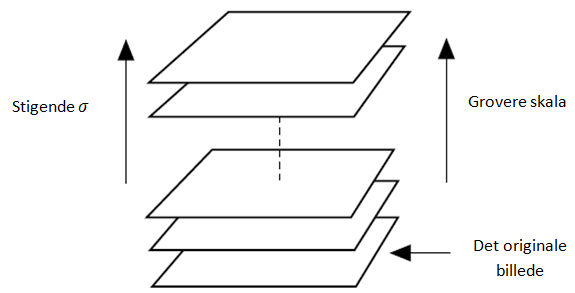
\includegraphics[width=0.55\textwidth]{fig/32.png}
     \vspace{-0.5em}
    \begin{center}    
       \caption{{\footnotesize \textit{En lineær skalarums repræsentation af et billede. Skalabillederne opstilles som en stak af billeder udsat for stigende grad af slørring}}}
    \label{fig:scalerep}
     \end{center}
     \vspace{-2.5em}
  \end{figure} \noindent
Denne overgang fra finere til grovere strukturer kan opnås ved systematisk at folde et billede med et Gaussisk filter af stigende sigmaværdi, hvor det nederste billede i stakken kan repræsenteres ved billedet $ L(x,y,0) = I(x,y)$ og for $\sigma>0$, defineres et skalabillede ved:
\begin{equation}
L(x,y,\sigma) = G(x,y,\sigma)\ast I(x,y)
\label{scalespace1}
\end{equation}
\\
Filteret der bruges til at oprette en skalarumsrepræsentation, skal opfylde følgende egenskaber:
\begin{itemize}
\item{Et lokalt ekstrema må ikke forøges når skalaparametren stiger. Dette medfører at støj i billedet ikke tilføjes, når skalaparametren stiger \cite{lindkth}.}
\item{Hvis hver udglatnings kerne er tilknyttet en skalaparameter, og to kerner foldes med hinanden, ønskes det at den resulterende kerne har en skalaparameter, lig med summen af de foregående skalaparametre \cite{springer}.
\begin{equation}
g(\cdot;\sigma_1) \ast g(\cdot;\sigma_2)=g(\cdot;\sigma_1+\sigma_2)
\label{semi}
\end{equation}
Ovenstående viser at alle skalarums transformationer er af samme familie. En skalarums repræsentation ved en grov skala $\sigma_2$, kan derved udledes, ved en repræsentation fra en finere skala:
\begin{equation}
g(\cdot;\sigma_2) = g(\cdot;\sigma_2-\sigma_1)\ast g(;\sigma_1)\text{,}\sigma_2>\sigma_1
\end{equation}}
\end{itemize}
Der anvendes et Gaussisk filter da den imødekommer begge ovenstående egenskaber. Ved et Gaussisk filter vil strukturer, der eksistere på grovere skalaer være simplificeringer af strukturer fra finere skalaer. Witkin \cite{witkins} beviste dette i tilfældet for én-dimensionsalle signaler illustreret i figur \ref{scalespace1}, der viser resultatet af at glatte et signal med et Gaussisk filter af stigende sigmaværdi. Det ses tydeligt, hvordan signalets underliggende grovere struktur bliver udtrykt og at finere strukturer undertrykkes.
\begin{figure}[H]
    \centering
    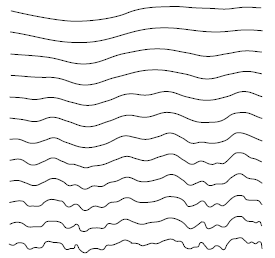
\includegraphics[width=0.45\textwidth]{fig/33.png}
     \vspace{-1em}
    \begin{center}    
       \caption{{\footnotesize \textit{Et én-dimensionalt signal udsat for et Gaussisk filter af gradvist stigende størrelse.}}}
    \label{fig:scalereps}
     \end{center}
     \vspace{-2.5em}
  \end{figure} \noindent
\subsubsection*{Skala Pyramide}
En udbredt metode, hvorpå skalarummet kan repræsenteres, er ved en \textit{skalapyramide}. Ved en skalapyramide repræsentation oprettes en pyramide af kopier af det undersøgte billede, hvor der for hvert niveau i pyramiden sker en reduktion af billedets størrelse, med en faktor af to. 
Når billedets størrelse skal halveres, er det ikke nok bare at fjerne hver anden række og hver anden kolonne, da dette vil resultere i store tab af billedets informationer. For at imødekomme dette problem, foldes billedet med et Gaussisk filter, inden billedet reduceres.  
Hvert niveau i pyramiden kaldes en oktav. Sigmaværdien fordobles imellem hver oktav.
 \begin{figure}[H]
    \centering
    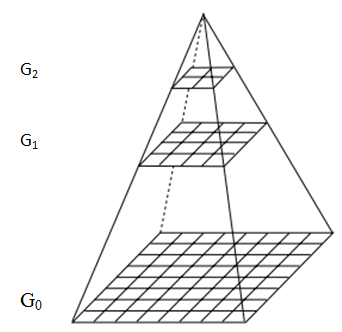
\includegraphics[width=0.40\textwidth]{fig/40.png}
     \vspace{-1em}
    \begin{center}    
       \caption{{\footnotesize \textit{En pyramiderepræsentation af et billede, der reduceres med en faktor af to, for hvert niveau. }}}
    \label{fig:scalerepdiff}
     \end{center}
     \vspace{-2.5em}
  \end{figure} \noindent
Hvis $G_0=I(x,y)$, kan de forskellige niveauer $l$ i skalapyramiden opnås ved:
\begin{equation}
G_l(i,j)=\sum\limits_{m}\sum\limits_{n}w(m,n)G_{l-1}(2i+m,2j+n)
\end{equation}
hvor $w$ er et Gaussisk filter. Fordelene ved en pyramiderepræsentation er at billedernes størrelser reduceres, hvilket reducere antallet af beregninger drastisk.